\documentclass{ucsdreport}

\graphicspath{{./images/}}
%************************************************************
% ABOUT THIS HOMEWORK
\def\course{ECE 269: Linear Algebra}                                        % Course
\def\thetitle{Orthogonal Matching Pursuit and Sparse Signal Recovery}       % Report Title
\def\Headauthor{Xingyi Yang}                                                % Header Authors of work
\def\date{\today}                                                           % Date

% DOCUMENT START
\begin{document}

\providecommand{\keywords}[1]{\textbf{\textit{Keywords---}} #1}
\theoremstyle{definition}
\newtheorem{definition}{Definition}[section]
\DeclarePairedDelimiter{\nint}\lfloor\rceil
% TITLE PAGE
\begin{center}
    \vspace*{1.5cm}
    % University Logo
    
\includegraphics[scale = 0.10]{UCSDseal.png}\\[1.75cm]
    % University Name
    \textsc{\color[RGB]{0, 51, 102}\LARGE{University of California San Diego}}\\[.5cm]
    \textsc{Jacob School of Engineering}\\[1cm]
    \textsc{\Large{\course}}\\[.5cm]
    \textsc{\Large{\thetitle}}\\[.5cm]
    \textsc{\date}\\[2cm]
    \Large{
    \begin{tabular}{L{4cm} R{4cm}}
        \textit{Author} &  \textit{Student ID}\\
        \hline
        % author names and PID
        Xingyi Yang & A53316455\\
    \end{tabular}
    }
\end{center}
\thispagestyle{empty}
\pagebreak

% TABLE OF CONTENTS
\tableofcontents{}
\pagebreak

% REPORT START
\section*{Abstract}
\addcontentsline{toc}{section}{Abstract}
Sparse approximation is the problem to find the sparsest linear combination for a signal from a redundant dictionary, which is widely applied in signal processing and compressed sensing. In this project, I manage to implement the Orthogonal Matching Pursuit (OMP) algorithm for sparse signals and images approximation. Meanwhile, this report analyses its performance under noiseless and noisy environments. 

\keywords{Orthogonal Matching Pursuit (OMP), Sparse Approximation, Signal Recovery}
    
% Section 1: Introduction (about some background concept and introduce the structure of this report)
\section{Introduction}
In the field of signal processing, it is the usual case to represent signal with a linear combination of set of $m$ unit vectors. When those vectors are orthonormal, this approximation can be regarded as projection of signal onto the subspace spanned by elements of this $m$ orthonormal basis. However, when those vectors are linear dependent, less than $m$ vectors is needed since $m-r$ non-independent elements can be represent by the other $r$ linear independent vectors. One of the application is

Under the assumption of a linear dependent set, or in other words, redundant dictionaries, finding the sparsest representation is called sparse approximation problem. It is easy to imagine that if $m$ orthonormal basis can perfectly approximate a signal, surely $m+1$ should not be worse. Though orthogonal basis is efficient in most case, a dictionary with linear dependent vectors can do even better. That's why sparse approximation is of great significance in signal processing.

On the other hand, the biggest challenge is the selection of the non-zeros elements in the sparse representation, which make sparse approximation a NP-hard problem. 

In this project, I implement the Orthogonal Matching Pursuit (OMP) algorithm to recover the signal with random generated dictionary. I also show its robustness under noiseless and noisy situation. Section 2 will clarify some basic concept I use in the experiment, mainly focusing on the process of OMP algorithm. Section 3 covers the experiment setup, also demonstrating the statistical result of experiments. The python code are attached in the Appendix part for reference.

% Section 2: Methodology (How does MP and OMP perform)
\section{Methodology}
\subsection{Basic Concepts}

\begin{definition}{\textit{Dictionary}}
A dictionary $D=\{\varphi\}^N_{l=1}$ in $\Re ^M$ is a collection $D \subset \Re^M$ of unit-norm vectors. A dictionary has the following properties:
\begin{itemize}
    \item The subscript of $D$ is $\Omega=\{1,2,\dots,N\}$
    \item $\forall l\in \Omega, \|\varphi_l\|_2 = 1$
    \item Elements of $D$ are called atoms.
    \item If $D$ is linearly dependent, the dictionary is redundant.
    \item Cardinality refer to the the size of set, denoted by $|\cdot|$. Clearly $|D|=|\Omega|=N$.
\end{itemize}
\end{definition}

\begin{definition}{\textit{Sparse Approximation Problems}}
Given a dictionary $D=\{\varphi\}^N_{l=1}$ and $N>s>1$. Assume $A=\begin{bmatrix}\varphi_1&\varphi_2&\dots&\varphi_N\end{bmatrix}$, solve
\begin{equation}
    \begin{aligned}
     & & \arg\min_x \|y-Ax\|_2 \\
     \text{s.t.} & & \|x\|_0=s
    \end{aligned}
\end{equation}
where $y$ is the measurement, $A \in R^{M\times N} $ is the measurement matrix. $\|\cdot\|_0$ and $\|\cdot\|_2$ refers to the $L_0$ and $L_2$ norm respectively.

The indices of the non-zero entries of $x$ is denoted by $S$, where $\forall i \in S, x_{i} \ne 0$. It is obvious that $|S|=\|x\|_0=s$.
\end{definition}

\subsection{Matching Pursuit}
If $D$ contains a large number of vectors (N is large), solving for the most sparse representation of $x$ is computationally unacceptable for practical applications.

In 1993, Mallat and Zhang \cite{mallat1993matching} proposed a greedy solution address the sparse approximation problem, called Matching Pursuit(MP). For a given measurement $y$ and a dictionary $D$, MP algorithm iteratively generates a sorted list of atom indices that correlates most strongly with the residual measurement, which form the suboptimal solution to the problem of sparse signal representation.
\begin{algorithm}
\caption{Matching Pursuit}\label{MP}

\BState \emph{Input}: Measurement $y$, measurement matrix $A=\begin{bmatrix}\varphi_1&\varphi_2&\dots&\varphi_N\end{bmatrix}$
\BState \emph{Output}: Recovered signal $x$, indices for corresponding atoms indexes $S$
\BState \emph{Initialization}: $r_1\gets y$, $n\gets 1$, $S \gets \{\}$, $x \gets zeroList(N)$

\begin{algorithmic}[1]
    \Function{MP}{}
    \While{ stop rule == False }
    \State Find $i^*_n \in \Omega$ that $i^*_n=\arg\max_i |\langle r_n,\varphi_i \rangle| $
    \State $S \gets S \cup i^*_n$
    \State $x_{i^*_n} \gets \langle r_n,\varphi_{i^*_n} \rangle$
    \State $r_{n+1} \gets r_{n} - \langle r_n,\varphi_{i^*_n} \rangle\varphi_{i^*_n}$
    \State $n \gets n+1$
    
    \State \Return $x,S$
\end{algorithmic}
\end{algorithm}
\newline
In Algorithm \ref{MP}, $r_n$ is the residual measurement at step $n$. $x_{i^*_n}$ is the coefficient corresponding to the $\varphi_{i^*_n}$ for the final linear combination term. MP is known as a Greedy Algorithm. At each step, MP only select the $i^*_n$ atom with the greatest inner product value with the residual measurement. Th value of $x_{i^*_n}$ is merely relied the atom $\varphi_{i^*_n}$ with no respect on the global optimal solution.

\subsection{Orthogonal Matching Pursuit}
In this section we give a detailed description of the orthogonal matching pursuit (OMP) algorithm. For
any subset $S \subset \Omega$, denote by $A(S)$ a submatrix of measurement matrix $A$
consisting of the columns $\varphi_i$ with $i\in S$. $x(S)$ is the subvector corresponding to $A(S)$. Thus, the OMP algorithm can be stated as follows.

\begin{algorithm}
\caption{Orthogonal Matching Pursuit}\label{OMP}

\BState \emph{Input}: Measurement $y$, measurement matrix $A=\begin{bmatrix}\varphi_1&\varphi_2&\dots&\varphi_N\end{bmatrix}$
\BState \emph{Output}: Recovered signal $x$, indices for corresponding atoms indexes $S$
\BState \emph{Initialization}: $r_1\gets y$, $n\gets 1$, $S \gets \{\}$, $x \gets zeroList(N)$

\begin{algorithmic}[1]
    \Function{OMP}{}
    \While{stop rule == False}
    \State Find $i^*_n \in \Omega$ that $i^*_n=\arg\max_i |\langle r_n,\varphi_i \rangle| $
    \State $S \gets S \cup i^*_n$
    \State $x \gets (A(S)^TA(S))^{-1}A(S)^Ty$
    \State $r_{n+1} \gets r_{n} - Ax$
    \State $n \gets n+1$
    
    \State \Return $x,S$
\end{algorithmic}
\end{algorithm}
The OMP is also a stepwise forward selection algorithm and is easy to implement. Followed by the same atom selection criteria as MP method, OMP differ from MP in that, at each step, OMP computes the least square solution for $y=A(S)x$ that $x = (A(S)^TA(S))^{-1}A(S)^Ty$. This least-squares minimization aims to obtain the best approximation over the atoms that have already been chosen. A superiority of OMP is that it never selects the same atom twice because the residual is orthogonal to the atoms that have already been chosen.

Another key component of OMP is the stopping rule which depends on the noise structure. In the noiseless case the natural stopping rule is $r_n=0$. In this project, we shall consider several different noise structures\cite{cai2011orthogonal}. To be more specific, two types of noise condition are considered. One is that when the sparsity $s=|S|$ is known, the iteration stops when $n \geq s$. Another situation stands for unknown sparsity but known norm bound. Under the second condition, the searching for $S$ stops when $\|r_n\|_2 \leq t$ where $r_n=y-Ax$. In
addition, we would mainly consider the important case of Gaussian
noise where $n \sim N(0,\sigma^2)$. The stopping rule for each case
and the properties of the resulting procedure will be discussed
in Section 3.
% Section 3: Experiment setup, Metrics and Results
\section{Experiment}
\subsection{Evaluation Metrics}
\paragraph{Normalized Error} Let $\hat{x}$ be the estimate of $x$ obtained from OMP. To measure the performance of OMP, we consider the Normalized Error defined as
\begin{align*}
    Normalized Error = \frac{\|x - \hat{x}\|_2}{\|x\|_2}
\end{align*}
The average Normalized Error is obtained by averaging the Normazlized Error over 2000 Monte Carlo runs.

\paragraph{Peak Signal-to-noise Ratio}Peak Signal-to-Noise ratio(PSNR) is widely used as image quality metric. Given a noise-free $m\times n$ monochrome image $I$ and its approximation $\hat{I}$, MSE is defined as:
\begin{align*}
    {MSE}={\frac {1}{m\,n}\sum _{i=0}^{m-1}\sum _{j=0}^{n-1}[I(i,j)-\hat{I}(i,j)]^{2}}
\end{align*}

The PSNR (in dB) is defined as:
\begin{align*}
    PSNR = 10\log_{10}(\frac{MAX_I^2}{MSE})
\end{align*}

Here, $MAX_I$ is the maximum possible pixel value of the image. When the pixels are represented using 8 bits per sample, this is 255. 

\paragraph{Exact Recovery for OMP} Without proof, a sufficient condition for OMP to recover the sparsest representation of the input signal is that
\begin{align*}
    \max_{l \not\in S }\|A(S)^+ \varphi_l\|_1<1
\end{align*}
where $A(s)^+ = (A^HA)^{-1}A^H$

\subsection{Experimental Setup}
In this project, we explore the performance and robustness of OMP algorithm under noiseless and noisy situation. Thus we design 6 set of experiments. The experiment details are elaborated below.
\begin{itemize}
    \item Noiseless case
    \begin{enumerate}
    
        \item \textbf{Noiseless phase transition plot with Exact Support Recovery probability} 
        
        With each $N \in \{20, 50, 100\}$, I vary $M$ and $s_{max}$ and calculate the probability of Exact Support Recovery by averaging over 2000 random realizations of $A \in \Re^{M \times N}$ and $x \in \Re^N$ with $s\sim U(1,s_{max})$ non-zero elements. The measurement $y$ is computed as
        \begin{align*}
            y = Ax
        \end{align*}
        In my implementation, $M \in \{10,15,20,\dots,95\}$ and $s_{max} \in \{\nint{\frac{N}{2}} ,\nint{\frac{N}{2}}+3, \nint{\frac{N}{2}}+6, \dots\}$($\max s_{max} < N$). $\nint{\cdot}$ refers to the round operation. Stop iteration when $\|r_n\|_2 \leq \epsilon=0.001$.
        
        \item \textbf{Noiseless phase transition plots with Normalized Error}
        
        With fixes $N \in \{20, 50, 100\}$, I vary $M$ and $s_{max}$ and calculate the Normalized Error by averaging over 2000 random realizations of $A \in \Re^{M \times N}$ and $x \in \Re^N$ with $s\sim U(1,s_{max})$ non-zero elements. The measurement $y$ is computed as
        \begin{align*}
            y = Ax
        \end{align*}
        In my implementation, $M \in \{10,15,20,\dots,95\}$ and $s_{max} \in \{\nint{\frac{N}{2}} ,\nint{\frac{N}{2}}+3, \nint{\frac{N}{2}}+6, \dots\}$($\max s_{max} < N$). Stop iteration when $\|r_n\|_2 \leq \epsilon=0.001$.
        
    \end{enumerate}
    \item Noisy case 
    \begin{enumerate}
    
        \item \textbf{Noisy phase transition with Normalized Error, known sparsity}
            
            With each $N \in \{20, 50, 100\}$, I vary $M$ and $s_{max}$ and calculate the probability of Successful Recovery ($Normalized Error < 0.001$) by averaging over 2000 random realizations of $A \in \Re^{M \times N}$ and $x \in \Re^N$ with $s\sim U(1,s_{max})$ non-zero elements. The noise vector is drawn form $N(0,\sigma^2)$, with $\sigma \in \{0.001, 0.01\}$. The measurement $y$ is computed as
        \begin{align*}
            y = Ax+n
        \end{align*}
            In my implementation, $M \in \{10,15,20,\dots,95\}$ and $s_{max} \in \{\nint{\frac{N}{2}} ,\nint{\frac{N}{2}}+3, \nint{\frac{N}{2}}+6, \dots\}$($\max s_{max} < N$). $\nint{\cdot}$ refers to the round operation. Stop iteration when $n=s$.
        
        \item \textbf{Noisy phase transition with Normalized Error, known noise norm}
        
            With each $N \in \{20, 50, 100\}$, I vary $M$ and $s_{max}$ and calculate the probability of Successful Recovery ($Normalized Error < 0.001$) by averaging over 2000 random realizations of $A \in \Re^{M \times N}$ and $x \in \Re^N$ with $s\sim U(1,s_{max})$ non-zero elements. The noise vector is drawn form $N(0,\sigma^2)$, with $\sigma \in \{0.001, 0.01\}$. The measurement $y$ is computed as
        \begin{align*}
            y = Ax+n
        \end{align*}
            In my implementation, $M \in \{10,15,20,\dots,95\}$ and $s_{max} \in \{\nint{\frac{N}{2}} ,\nint{\frac{N}{2}}+3, \nint{\frac{N}{2}}+6, \dots\}$($\max s_{max} < N$). $\nint{\cdot}$ refers to the round operation. Stop iteration when $\|r_n\|_2 \leq \|n\|_2$.
            
    \end{enumerate}
    \item Image case
    \begin{enumerate}
        \item \textbf{Noiseless image recovery}
        
        The original image is processed by Discrete Cosine Transform(DCT) with $8\times 8$ blocks. Each $8\times 8$ DCT block is vectorize to a 64-dimension vector $x^{(i)}$ with zigzag pattern. Assume $x^{(i)} \in \Re^{64}$ as the ground-truth signal ($N=64$). I vary $M$ and randomly construct a $A \in \Re^{M \times 64}$ for the whole image at a time. The measurement $y^{(i)}$ for each vector is computed as
        \begin{align*}
            y^{(i)} = Ax^{(i)}
        \end{align*}
        Each reconstructed signal $\hat{x}^{(i)}$ is reshaped into $8 \times 8$ and inverse discrete cosine transformed (IDCT) to a image block. I repeat the image reconstruction over 100 times and calculate the Normalized Error and PSNR to evaluate the recovery performance of OMP algorithm. In my implementation, $M \in \{10,15,20,\dots,95\}$ and the Stop rule is $\|r_n\|_2 \leq \epsilon=0.001$.
        
        \item \textbf{Noisy image recovery}
        
        The original image is processed by Discrete Cosine Transform(DCT) with $8\times 8$ blocks. Each $8\times 8$ DCT block is vectorize to a 64-dimension vector $x^{(i)}$ with zigzag pattern. Assume $x^{(i)} \in \Re^{64}$ as the ground-truth signal ($N=64$). I vary $M$ and randomly construct a $A \in \Re^{M \times 64}$ for the whole image at a time. The noise vector $n^{(i)}$ is drawn form $N(0,\sigma^2)$, with $\sigma \in \{0.001, 0.01\}$. The measurement $y^{(i)}$ for each vector is computed as
        \begin{align*}
            y^{(i)} = Ax^{(i)}+n^{(i)}
        \end{align*}
        Each reconstructed signal $\hat{x}^{(i)}$ is reshaped into $8 \times 8$ and inverse discrete cosine transformed (IDCT) to a image block. I repeat the image reconstruction over 100 times and calculate the Normalized Error and PSNR to evaluate the recovery performance of OMP algorithm. In my implementation, $M \in \{10,15,20,\dots,95\}$ and the Stop rule is $\|r_n\|_2 \leq \|n\|_2$.
    \end{enumerate}
\end{itemize}
The two experiment under Noiseless Case study the relation between recovery performance and various $M$ and $s_{max}$. Two Noisy experiments compare the robustness of OMP algorithm under different noise degree and with different stop rule. Image recovery tests the ability of OMP method in terms of practical application.

\subsection{Main Result}
\subsubsection{Noiseless Case}
The Noiseless phase transition plot with $N\in \{20,50,100\}$ are displayed in Fig.\ref{fig:Noiseless}. Under the noiseless situation, we can see that Normalized Error sharply drops with the increase of both $M$ and $s_{max}$, where as the the success probability of Exact Support Recovery gradually reach to 1. We may observe a sharp transition region where both the probability of ESR and average Normalized Error quickly transitions. This transition approximately happens around $M=N$. When $N>M$ the normalized error tends to be large and the successful probability is quite low. This phenomenon results in that, for Fig.\ref{fig:NoiselessNorm20}\ref{fig:NoiselessESR20} where $N=20$, most of the experiments are of good performance. However from Fig.\ref{fig:NoiselessNorm100}\ref{fig:NoiselessESR100}, The recovery result for large $N$ is poor.
\begin{figure}[h]
    \centering
    \subfigure[Normalized Error N=20]{
    \includegraphics[width=0.48\textwidth]{images/Noiseless/N20.png}
    \label{fig:NoiselessNorm20}
    }
    \subfigure[Probability of Exact Support Recovery N=20]{
    \includegraphics[width=0.48\textwidth]{images/Noiseless/N20_ESR_rate.png}
    \label{fig:NoiselessESR20}
    }
    \subfigure[Normalized Error N=50]{
    \includegraphics[width=0.48\textwidth]{images/Noiseless/N50.png}
    \label{fig:NoiselessNorm50}
    }
    \subfigure[Probability of Exact Support Recovery N=50]{
    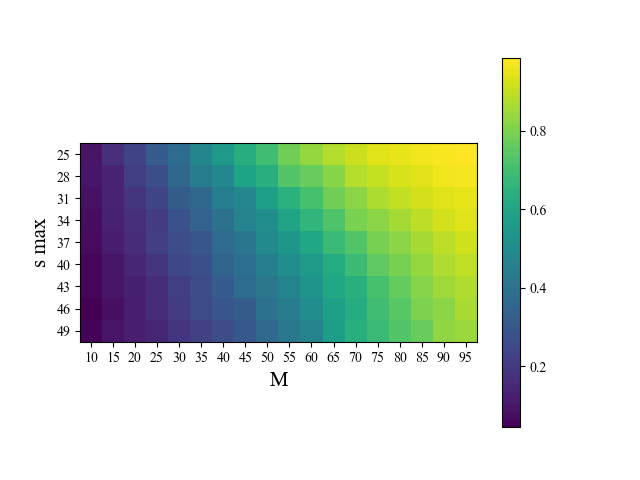
\includegraphics[width=0.48\textwidth]{images/Noiseless/N50_ESR_rate.png}
    \label{fig:NoiselessESR50}
    }
    \subfigure[Normalized Error N=100]{
    \includegraphics[width=0.48\textwidth]{images/Noiseless/N100.png}
    \label{fig:NoiselessNorm100}
    }
    \subfigure[Probability of Exact Support Recovery N=100]{
    \includegraphics[width=0.48\textwidth]{images/Noiseless/N100_ESR_rate.png}
    \label{fig:NoiselessESR100}
    }
    \caption{Noiseless phase transition plot with different N}
    \label{fig:Noiseless}
\end{figure}
\subsubsection{Noisy Case}
\begin{figure}[h]
    \centering
    \subfigure[$\sigma=0.001$ and $N=20$]{
    \includegraphics[width=0.3\textwidth]{images/Noise1/Noise1_N20_sigma10-3.png}
    \label{fig:Noise1Norm2010-3}
    }
    \subfigure[$\sigma=0.001$ and $N=50$]{
    \includegraphics[width=0.3\textwidth]{images/Noise1/Noise1_N50_sigma10-3.png}
    \label{fig:Noise1Norm5010-3}
    }
    \subfigure[$\sigma=0.001$ and $N=100$]{
    \includegraphics[width=0.3\textwidth]{images/Noise1/Noise1_N100_sigma10-3.png}
    \label{fig:Noise1Norm10010-3}
    }
    \subfigure[$\sigma=0.01$ and $N=20$]{
    \includegraphics[width=0.3\textwidth]{images/Noise1/Noise1_N20_sigma10-2.png}
    \label{fig:Noise1Norm2010-2}
    }
    \subfigure[$\sigma=0.01$ and $N=50$]{
    \includegraphics[width=0.3\textwidth]{images/Noise1/Noise1_N50_sigma10-2.png}
    \label{fig:Noise1Norm5010-2}
    }
    \subfigure[$\sigma=0.01$ and $N=100$]{
    \includegraphics[width=0.3\textwidth]{images/Noise1/Noise1_N100_sigma10-2.png}
    \label{fig:Noise1Norm10010-2}
    }
    \caption{Noisy phase transition plot, known sparsity}
    \label{fig:Noise1}
\end{figure}

\begin{figure}[h]
    \centering
    \subfigure[$\sigma=0.001$ and $N=20$]{
    \includegraphics[width=0.3\textwidth]{images/Noise2/Noise2_N20_sigma10-3.png}
    \label{fig:Noise2Norm2010-3}
    }
    \subfigure[$\sigma=0.001$ and $N=50$]{
    \includegraphics[width=0.3\textwidth]{images/Noise2/Noise2_N50_sigma10-3.png}
    \label{fig:Noise2Norm5010-3}
    }
    \subfigure[$\sigma=0.001$ and $N=100$]{
    \includegraphics[width=0.3\textwidth]{images/Noise2/Noise2_N100_sigma10-3.png}
    \label{fig:Noise2Norm10010-3}
    }
    \subfigure[$\sigma=0.01$ and $N=20$]{
    \includegraphics[width=0.3\textwidth]{images/Noise2/Noise2_N20_sigma10-2.png}
    \label{fig:Noise2Norm2010-2}
    }
    \subfigure[$\sigma=0.01$ and $N=50$]{
    \includegraphics[width=0.3\textwidth]{images/Noise2/Noise2_N50_sigma10-2.png}
    \label{fig:Noise2Norm5010-2}
    }
    \subfigure[$\sigma=0.01$ and $N=100$]{
    \includegraphics[width=0.3\textwidth]{images/Noise2/Noise2_N100_sigma10-2.png}
    \label{fig:Noise2Norm10010-2}
    }
    \caption{Noisy phase transition plot, known noise norm}
    \label{fig:Noise2}
\end{figure}
It is the usual case that that a signal may suffer from unwanted noise during capture, storage, transmission, processing, or conversion. In this section, we intentionally add noise to the measurement with different assumptions to testify the robustness of the OMP algorithm.
\paragraph{Noisy measurement with known sparsity} Under the assumption of known sparsity, the iterations for atom selection stop when $n\geq r$. The probability of successful recovery under different $M$ and $s_{max}$ is shown in Fig.\ref{fig:Noise1}. With small $\sigma=0.001$, the OMP algorithm still performs considerably robustly, resembling the noiseless situation. In Fig.\ref{fig:Noise1Norm2010-3}, when $M >> N$, most signals can be successfully reconstructed the probability is approximately above 0.9. However, when the noise's variance grows to $0.01$, the recovery performance messed up. As we may noitice in Fig.\ref{fig:Noise1Norm2010-2}\ref{fig:Noise1Norm5010-2}\ref{fig:Noise1Norm10010-2}, no matter how $M$ increases, the successful rate is under 0.2.
\paragraph{Noisy measurement with known noise norm}
\subsubsection{Image Case}

% Section 4: Conclusion
\section{Conclusion}

% Reference

\addcontentsline{toc}{section}{Reference}

\bibliographystyle{plain}
\bibliography{cfg/mybib}

% Appendix: Code
\section*{Appendix}
\addcontentsline{toc}{section}{Appendix}
%************************************************************
\end{document}